%%%% Paramétrage du TD %%%%
\def\xxactivite{TD 1 \ifprof -- Corrigé \else \fi} % \normalsize \vspace{-.4cm}
\def\xxauteur{\textsl{Xavier Pessoles}}


\def\xxnumchapitre{Chapitre 1 \vspace{.2cm}}
\def\xxchapitre{\hspace{.12cm} Correction des systèmes}


\def\xxcompetences{%
\vspace{-.3cm}
\textsl{%
\textbf{Savoirs et compétences :}\\
\vspace{-.4cm}
\begin{itemize}[label=\ding{112},font=\color{ocre}] 
%\item \textit{Res1.C4 : } Correction
\item \textit{Res1.C4.SF1 : } Proposer la démarche de réglage d’un correcteur proportionnel, 
proportionnel intégral 
%et à avance de phase
\item \textit{Con.C2 : } 	Correction d’un système asservi	
%\item \textit{Con.C2.SF1 : } Choisir un type de correcteur adapté
\end{itemize}
}}

\def\xxtitreexo{La robotique au service du handicap}
\def\xxsourceexo{\hspace{.2cm} Centrale Supélec -- PSI 2010}
\def\xxauteur{\textsl{Xavier Pessoles}}

\def\xxfigures{
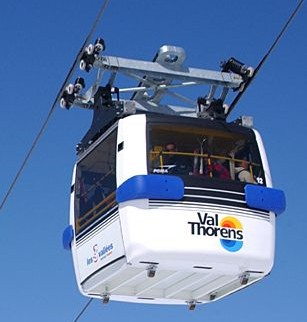
\includegraphics[width=.35\linewidth]{fig_00}
}%figues de la page de garde


\iflivret
\pagestyle{empty}


%%%%%%%% PAGE DE GARDE COURS
\ifcours
\begin{tikzpicture}[remember picture,overlay]
\node at (current page.north west)
{\begin{tikzpicture}[remember picture,overlay]
\node[anchor=north west,inner sep=0pt] at (0,0) {\includegraphics[width=\paperwidth]{\thechapterimage}};
\draw[anchor=west] (-2cm,-8cm) node [line width=2pt,rounded corners=15pt,draw=ocre,fill=white,fill opacity=0.6,inner sep=40pt]{\strut\makebox[22cm]{}};
\draw[anchor=west] (1cm,-8cm) node {\huge\sffamily\bfseries\color{black} %
\begin{minipage}{1cm}
\rotatebox{90}{\LARGE\sffamily\textsc{\color{ocre}\textbf{\xxnumpartie}}}
\end{minipage} \hfill
\begin{minipage}[c]{14cm}
\begin{titrepartie}
\begin{flushright}
\renewcommand{\baselinestretch}{1.1} 
\Large\sffamily\textsc{\textbf{\xxpartie}}
\renewcommand{\baselinestretch}{1} 
\end{flushright}
\end{titrepartie}
\end{minipage} \hfill
\begin{minipage}[c]{3.5cm}
{\large\sffamily\textsc{\textbf{\color{ocre} \discipline}}}
\end{minipage} 
 };
\end{tikzpicture}};
\end{tikzpicture}


\begin{tikzpicture}[overlay]
\node[shape=rectangle, 
      rounded corners = .25 cm,
	  draw= ocre,
	  line width=2pt, 
	  fill = ocre!10,
	  minimum width  = 2.5cm,
	  minimum height = 3cm,] at (18cm,0) {};
\node at (17.7cm,0) {\rotatebox{90}{\textbf{\Large\color{ocre}{\classe}}}};
%{};
\end{tikzpicture}

\vspace{3.5cm}

\begin{tikzpicture}[remember picture,overlay]
\draw[anchor=west] (-2cm,-6cm) node {\huge\sffamily\bfseries\color{black} %
\begin{minipage}{2cm}
\begin{center}
\LARGE\sffamily\textsc{\color{ocre}\textbf{\xxactivite}}
\end{center}
\end{minipage} \hfill
\begin{minipage}[c]{15cm}
\begin{titrechapitre}
\renewcommand{\baselinestretch}{1.1} 
\Large\sffamily\textsc{\textbf{\xxnumchapitre}}

\Large\sffamily\textsc{\textbf{\xxchapitre}}
\vspace{.5cm}

\renewcommand{\baselinestretch}{1} 
\normalsize\normalfont
\xxcompetences
\end{titrechapitre}
\end{minipage}  };
\end{tikzpicture}
\vfill

\begin{flushright}
\begin{minipage}[c]{.3\linewidth}
\begin{center}
\xxfigures
\end{center}
\end{minipage}\hfill
\begin{minipage}[c]{.6\linewidth}
\startcontents
\printcontents{}{1}{}
\end{minipage}
\end{flushright}

\begin{tikzpicture}[remember picture,overlay]
\draw[anchor=west] (4.5cm,-.7cm) node {
\begin{minipage}[c]{.2\linewidth}
\begin{flushright}

\includegraphics[width=2cm]{png/logoCC}
\end{flushright}
\end{minipage}
\begin{minipage}[c]{.2\linewidth}
\textsl{\xxauteur} \\
\textsl{\classe}
\end{minipage}
 };
\end{tikzpicture}
\newpage
\pagestyle{fancy}

\newpage
\pagestyle{fancy}

\else
\fi


%%%%%%%% PAGE DE GARDE TD
\iftd
%\begin{tikzpicture}[remember picture,overlay]
%\node at (current page.north west)
%{\begin{tikzpicture}[remember picture,overlay]
%\draw[anchor=west] (-2cm,-3.25cm) node [line width=2pt,rounded corners=15pt,draw=ocre,fill=white,fill opacity=0.6,inner sep=40pt]{\strut\makebox[22cm]{}};
%\draw[anchor=west] (1cm,-3.25cm) node {\huge\sffamily\bfseries\color{black} %
%\begin{minipage}{1cm}
%\rotatebox{90}{\LARGE\sffamily\textsc{\color{ocre}\textbf{\xxnumpartie}}}
%\end{minipage} \hfill
%\begin{minipage}[c]{13.5cm}
%\begin{titrepartie}
%\begin{flushright}
%\renewcommand{\baselinestretch}{1.1} 
%\Large\sffamily\textsc{\textbf{\xxpartie}}
%\renewcommand{\baselinestretch}{1} 
%\end{flushright}
%\end{titrepartie}
%\end{minipage} \hfill
%\begin{minipage}[c]{3.5cm}
%{\large\sffamily\textsc{\textbf{\color{ocre} \discipline}}}
%\end{minipage} 
% };
%\end{tikzpicture}};
%\end{tikzpicture}

%%%%%%%%%% PAGE DE GARDE TD %%%%%%%%%%%%%%%
%\begin{tikzpicture}[overlay]
%\node[shape=rectangle, 
%      rounded corners = .25 cm,
%	  draw= ocre,
%	  line width=2pt, 
%	  fill = ocre!10,
%	  minimum width  = 2.5cm,
%	  minimum height = 2.5cm,] at (18.5cm,0) {};
%\node at (17.7cm,0) {\rotatebox{90}{\textbf{\Large\color{ocre}{\classe}}}};
%%{};
%\end{tikzpicture}

% PARTIE ET CHAPITRE
%\begin{tikzpicture}[remember picture,overlay]
%\draw[anchor=west] (-1cm,-2.1cm) node {\large\sffamily\bfseries\color{black} %
%\begin{minipage}[c]{15cm}
%\begin{flushleft}
%\xxnumchapitre \\
%\xxchapitre
%\end{flushleft}
%\end{minipage}  };
%\end{tikzpicture}

% Bandeau titre exo
\begin{tikzpicture}[remember picture,overlay]
\draw[anchor=west] (-2cm,-6cm) node {\huge\sffamily\bfseries\color{black} %
\begin{minipage}{5cm}
\begin{center}
\LARGE\sffamily\color{ocre}\textbf{\textsc{\xxactivite}}

\begin{center}
\xxfigures
\end{center}

\end{center}
\end{minipage} \hfill
\begin{minipage}[c]{12cm}
\begin{titrechapitre}
\renewcommand{\baselinestretch}{1.1} 
\large\sffamily\textbf{\textsc{\xxtitreexo}}

\small\sffamily{\textbf{\textit{\color{black!70}\xxsourceexo}}}
\vspace{.5cm}

\renewcommand{\baselinestretch}{1} 
\normalsize\normalfont
\xxcompetences
\end{titrechapitre}
\end{minipage}  };
\end{tikzpicture}

\else
\fi


%%%%%%%% PAGE DE GARDE FICHE
\iffiche
\begin{tikzpicture}[remember picture,overlay]
\node at (current page.north west)
{\begin{tikzpicture}[remember picture,overlay]
\draw[anchor=west] (-2cm,-3.25cm) node [line width=2pt,rounded corners=15pt,draw=ocre,fill=white,fill opacity=0.6,inner sep=40pt]{\strut\makebox[22cm]{}};
\draw[anchor=west] (1cm,-3.25cm) node {\huge\sffamily\bfseries\color{black} %
\begin{minipage}{1cm}
\rotatebox{90}{\LARGE\sffamily\textsc{\color{ocre}\textbf{\xxnumpartie}}}
\end{minipage} \hfill
\begin{minipage}[c]{14cm}
\begin{titrepartie}
\begin{flushright}
\renewcommand{\baselinestretch}{1.1} 
\large\sffamily\textsc{\textbf{\xxpartie} \\} 

\vspace{.2cm}

\normalsize\sffamily\textsc{\textbf{\xxnumchapitre -- \xxchapitre}}
\renewcommand{\baselinestretch}{1} 
\end{flushright}
\end{titrepartie}
\end{minipage} \hfill
\begin{minipage}[c]{3.5cm}
{\large\sffamily\textsc{\textbf{\color{ocre} \discipline}}}
\end{minipage} 
 };
\end{tikzpicture}};
\end{tikzpicture}


\begin{tikzpicture}[overlay]
\node[shape=rectangle, 
      rounded corners = .25 cm,
	  draw= ocre,
	  line width=2pt, 
	  fill = ocre!10,
	  minimum width  = 2.5cm,
%	  minimum height = 2.5cm,] at (18.5cm,0.5cm) {};
	  minimum height = 2.5cm,] at (18.5cm,0cm) {};
\node at (17.7cm,0) {\rotatebox{90}{\textsf{\textbf{\large\color{ocre}{\classe}}}}};
%{};
\end{tikzpicture}



\else
\fi



\else
\pagestyle{empty}


%%%%%%%% PAGE DE GARDE COURS
\ifcours
\begin{tikzpicture}[remember picture,overlay]
\node at (current page.north west)
{\begin{tikzpicture}[remember picture,overlay]
\node[anchor=north west,inner sep=0pt] at (0,0) {\includegraphics[width=\paperwidth]{\thechapterimage}};
\draw[anchor=west] (-2cm,-8cm) node [line width=2pt,rounded corners=15pt,draw=ocre,fill=white,fill opacity=0.6,inner sep=40pt]{\strut\makebox[22cm]{}};
\draw[anchor=west] (1cm,-8cm) node {\huge\sffamily\bfseries\color{black} %
\begin{minipage}{1cm}
\rotatebox{90}{\LARGE\sffamily\textsc{\color{ocre}\textbf{\xxnumpartie}}}
\end{minipage} \hfill
\begin{minipage}[c]{14cm}
\begin{titrepartie}
\begin{flushright}
\renewcommand{\baselinestretch}{1.1} 
\Large\sffamily\textsc{\textbf{\xxpartie}}
\renewcommand{\baselinestretch}{1} 
\end{flushright}
\end{titrepartie}
\end{minipage} \hfill
\begin{minipage}[c]{3.5cm}
{\large\sffamily\textsc{\textbf{\color{ocre} \discipline}}}
\end{minipage} 
 };
\end{tikzpicture}};
\end{tikzpicture}


\begin{tikzpicture}[overlay]
\node[shape=rectangle, 
      rounded corners = .25 cm,
	  draw= ocre,
	  line width=2pt, 
	  fill = ocre!10,
	  minimum width  = 2.5cm,
	  minimum height = 3cm,] at (18cm,0) {};
\node at (17.7cm,0) {\rotatebox{90}{\textbf{\Large\color{ocre}{\classe}}}};
%{};
\end{tikzpicture}

\vspace{3.5cm}

\begin{tikzpicture}[remember picture,overlay]
\draw[anchor=west] (-2cm,-6cm) node {\huge\sffamily\bfseries\color{black} %
\begin{minipage}{2cm}
\begin{center}
\LARGE\sffamily\textsc{\color{ocre}\textbf{\xxactivite}}
\end{center}
\end{minipage} \hfill
\begin{minipage}[c]{15cm}
\begin{titrechapitre}
\renewcommand{\baselinestretch}{1.1} 
\Large\sffamily\textsc{\textbf{\xxnumchapitre}}

\Large\sffamily\textsc{\textbf{\xxchapitre}}
\vspace{.5cm}

\renewcommand{\baselinestretch}{1} 
\normalsize\normalfont
\xxcompetences
\end{titrechapitre}
\end{minipage}  };
\end{tikzpicture}
\vfill

\begin{flushright}
\begin{minipage}[c]{.3\linewidth}
\begin{center}
\xxfigures
\end{center}
\end{minipage}\hfill
\begin{minipage}[c]{.6\linewidth}
\startcontents
\printcontents{}{1}{}
\end{minipage}
\end{flushright}

\begin{tikzpicture}[remember picture,overlay]
\draw[anchor=west] (4.5cm,-.7cm) node {
\begin{minipage}[c]{.2\linewidth}
\begin{flushright}

\includegraphics[width=2cm]{png/logoCC}
\end{flushright}
\end{minipage}
\begin{minipage}[c]{.2\linewidth}
\textsl{\xxauteur} \\
\textsl{\classe}
\end{minipage}
 };
\end{tikzpicture}
\newpage
\pagestyle{fancy}

\newpage
\pagestyle{fancy}

\else
\fi


%%%%%%%% PAGE DE GARDE TD
\iftd
%\begin{tikzpicture}[remember picture,overlay]
%\node at (current page.north west)
%{\begin{tikzpicture}[remember picture,overlay]
%\draw[anchor=west] (-2cm,-3.25cm) node [line width=2pt,rounded corners=15pt,draw=ocre,fill=white,fill opacity=0.6,inner sep=40pt]{\strut\makebox[22cm]{}};
%\draw[anchor=west] (1cm,-3.25cm) node {\huge\sffamily\bfseries\color{black} %
%\begin{minipage}{1cm}
%\rotatebox{90}{\LARGE\sffamily\textsc{\color{ocre}\textbf{\xxnumpartie}}}
%\end{minipage} \hfill
%\begin{minipage}[c]{13.5cm}
%\begin{titrepartie}
%\begin{flushright}
%\renewcommand{\baselinestretch}{1.1} 
%\Large\sffamily\textsc{\textbf{\xxpartie}}
%\renewcommand{\baselinestretch}{1} 
%\end{flushright}
%\end{titrepartie}
%\end{minipage} \hfill
%\begin{minipage}[c]{3.5cm}
%{\large\sffamily\textsc{\textbf{\color{ocre} \discipline}}}
%\end{minipage} 
% };
%\end{tikzpicture}};
%\end{tikzpicture}

%%%%%%%%%% PAGE DE GARDE TD %%%%%%%%%%%%%%%
%\begin{tikzpicture}[overlay]
%\node[shape=rectangle, 
%      rounded corners = .25 cm,
%	  draw= ocre,
%	  line width=2pt, 
%	  fill = ocre!10,
%	  minimum width  = 2.5cm,
%	  minimum height = 2.5cm,] at (18.5cm,0) {};
%\node at (17.7cm,0) {\rotatebox{90}{\textbf{\Large\color{ocre}{\classe}}}};
%%{};
%\end{tikzpicture}

% PARTIE ET CHAPITRE
%\begin{tikzpicture}[remember picture,overlay]
%\draw[anchor=west] (-1cm,-2.1cm) node {\large\sffamily\bfseries\color{black} %
%\begin{minipage}[c]{15cm}
%\begin{flushleft}
%\xxnumchapitre \\
%\xxchapitre
%\end{flushleft}
%\end{minipage}  };
%\end{tikzpicture}

% Bandeau titre exo
\begin{tikzpicture}[remember picture,overlay]
\draw[anchor=west] (-2cm,-6cm) node {\huge\sffamily\bfseries\color{black} %
\begin{minipage}{5cm}
\begin{center}
\LARGE\sffamily\color{ocre}\textbf{\textsc{\xxactivite}}

\begin{center}
\xxfigures
\end{center}

\end{center}
\end{minipage} \hfill
\begin{minipage}[c]{12cm}
\begin{titrechapitre}
\renewcommand{\baselinestretch}{1.1} 
\large\sffamily\textbf{\textsc{\xxtitreexo}}

\small\sffamily{\textbf{\textit{\color{black!70}\xxsourceexo}}}
\vspace{.5cm}

\renewcommand{\baselinestretch}{1} 
\normalsize\normalfont
\xxcompetences
\end{titrechapitre}
\end{minipage}  };
\end{tikzpicture}

\else
\fi


%%%%%%%% PAGE DE GARDE FICHE
\iffiche
\begin{tikzpicture}[remember picture,overlay]
\node at (current page.north west)
{\begin{tikzpicture}[remember picture,overlay]
\draw[anchor=west] (-2cm,-3.25cm) node [line width=2pt,rounded corners=15pt,draw=ocre,fill=white,fill opacity=0.6,inner sep=40pt]{\strut\makebox[22cm]{}};
\draw[anchor=west] (1cm,-3.25cm) node {\huge\sffamily\bfseries\color{black} %
\begin{minipage}{1cm}
\rotatebox{90}{\LARGE\sffamily\textsc{\color{ocre}\textbf{\xxnumpartie}}}
\end{minipage} \hfill
\begin{minipage}[c]{14cm}
\begin{titrepartie}
\begin{flushright}
\renewcommand{\baselinestretch}{1.1} 
\large\sffamily\textsc{\textbf{\xxpartie} \\} 

\vspace{.2cm}

\normalsize\sffamily\textsc{\textbf{\xxnumchapitre -- \xxchapitre}}
\renewcommand{\baselinestretch}{1} 
\end{flushright}
\end{titrepartie}
\end{minipage} \hfill
\begin{minipage}[c]{3.5cm}
{\large\sffamily\textsc{\textbf{\color{ocre} \discipline}}}
\end{minipage} 
 };
\end{tikzpicture}};
\end{tikzpicture}


\begin{tikzpicture}[overlay]
\node[shape=rectangle, 
      rounded corners = .25 cm,
	  draw= ocre,
	  line width=2pt, 
	  fill = ocre!10,
	  minimum width  = 2.5cm,
%	  minimum height = 2.5cm,] at (18.5cm,0.5cm) {};
	  minimum height = 2.5cm,] at (18.5cm,0cm) {};
\node at (17.7cm,0) {\rotatebox{90}{\textsf{\textbf{\large\color{ocre}{\classe}}}}};
%{};
\end{tikzpicture}



\else
\fi



\fi
\setlength{\columnseprule}{.1pt}

\pagestyle{fancy}
\thispagestyle{plain}

\vspace{4.9cm}

\def\columnseprulecolor{\color{ocre}}
\setlength{\columnseprule}{0.4pt} 

%%%%%%%%%%%%%%%%%%%%%%%

\setcounter{exo}{0}
\begin{multicols}{2}

%\section*{}

\subsection*{Synthèse d’une loi de commande pour l’exosquelette}

\begin{obj}
L’objectif de cette partie est de mettre en place une loi de commande utilisée, par exemple, pour des
situations de travail où le patient peut déplacer le bras et doit appliquer une force prédéterminée par le
physiothérapeute, dépendante des positions des articulations. Dans le cadre de cette étude, l’effort est
élastique et caractérisé par une raideur de torsion. La synthèse de cette loi de commande sera faite en
deux étapes : dans un premier temps, la mise en équation de l’exosquelette (limité à deux axes pour des
raisons de simplicité) sera effectuée en vue d’obtenir un modèle dynamique ; dans un deuxième temps,
la loi de commande sera déterminée en utilisant le modèle dynamique établi au préalable. Il s’agira, de
plus, de valider le dimensionnement de la chaîne de motorisation.
\end{obj}

Le cahier des charges est rappelé partiellement par les exigences données dans le tableau suivant. Les actionneurs peuvent fournir, en régime permanent, sur l’axe de l’articulation un
couple de module inférieur à \SI{50}{Nm}. On suppose qu’en régime transitoire le couple maximal peut atteindre quatre fois la valeur maximale autorisée en régime permanent.

La structure des axes étudiés est donnée dans la figure suivante.

\begin{center}
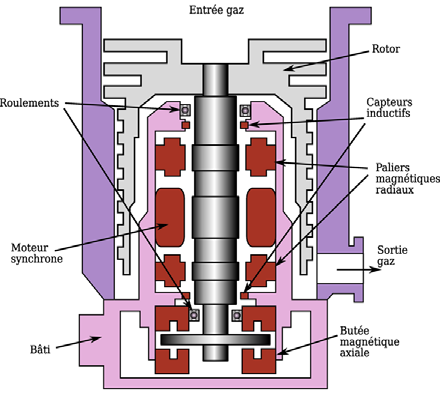
\includegraphics[width=1.0\linewidth]{fig_05}
\end{center}



On s’intéresse ici à une situation de travail où les relations entre les variations des positions angulaires du
bras et de l’avant bras $ ^t(\gamma,\delta)$ et de la variation de force $Z_F$ exercée par le patient sont équivalentes à des raideurs de torsion de valeurs $(K_1,K_2)$.


\begin{center}
\begin{tabular}{|p{.45\linewidth}|p{.45\linewidth}|}
\hline
Module de l’effort de manipulation maximal en régime permanent & \SI{50}{N} \\
\hline
Compensation du couple statique (dû à la pesanteur) & Totale \\ \hline
Raideurs $(K_1,K_2)$ de maintien (pour ce critère, seule la force $Z_F$ est
considérée) & $\left | \Delta Z_F / \Delta \gamma \right | = K_1 > \SI{500}{N.rad^{-1}}$ $(\pm\,5\%)$ 
$\left | \Delta Z_F / \Delta \delta \right  | = K_2 > \SI{500}{N.rad^{-1}}$ $(\pm\,5\%)$ \\
\hline
\end{tabular}
\end{center}


La structure de commande retenue est représentée par le schéma de la figure suivante où :
\begin{itemize}
\item $q$ et $\dot{q}$ sont respectivement les vecteurs des angles et des vitesses angulaires des articulations ;
\item une boucle externe génère les trajectoires (positions, vitesses et accélérations) et éventuellement un contexte de travail ;
\item une boucle interne (de loi non linéaire) génère les couples souhaités sur chaque axe (articulation) à partir des mesures des angles et des vitesses angulaires des articulations et éventuellement des données issues du générateur de trajectoire ;
\item  un ensemble d’actionneurs fournit les couples, sur les axes des articulations, identiques aux couples de
référence $C_a = C_{\text{ref}}$ .
\end{itemize}

\begin{center}
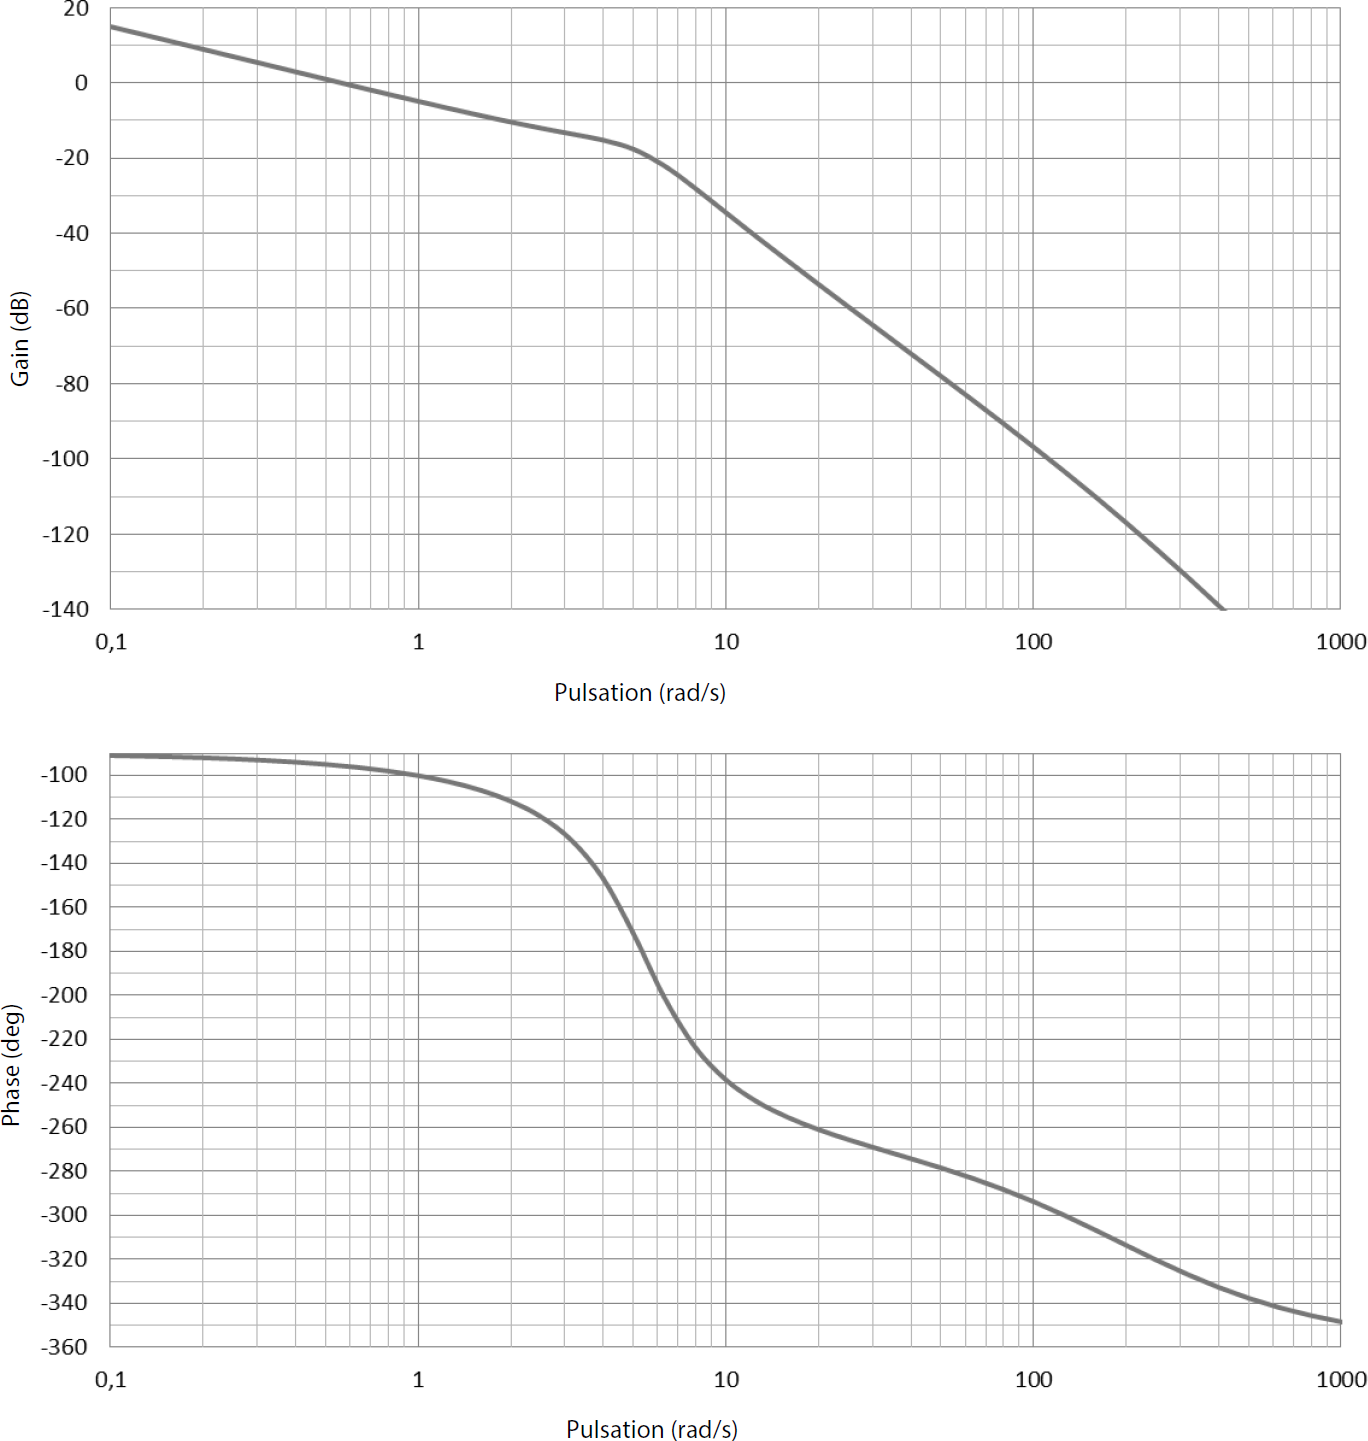
\includegraphics[width=1.0\linewidth]{fig_04}
\end{center}

\newpage

\subsection*{Modélisation dynamique «deux axes» de l’exosquelette}

\begin{obj}
Le but de cette partie est d’établir un modèle dynamique du bras et de l’avant-bras dans un plan vertical
donné. Ces deux ensembles sont soumis aux actions de la pesanteur, des couples des deux moteurs montés
dans le bras et de la force extérieure exercée sur l’extrémité de l’avant-bras. Le cadre de l’étude se limite
aux mouvements de deux axes (les deux autres axes étant supposés fixes).
\end{obj}

L’action du patient sur l’avant-bras, modélisée par une force appliquée à l’extrémité $B$ de l’avant-bras et
définie par : 
$\torseurstat{T}{\text{Force}}{\text{Avant-bras}}=\torseurl{X_F\vect{x}+Z_F\vect{z}}{\vect{0}}{B}$. 
L’action du premier actionneur sur le solide \{Bras\} : $\torseurstat{T}{\text{Actionneur 1}}{\text{Bras}}=\torseurl{\vect{0}}{C_1(t) \vect{y}}{O}$ où le couple $C_1(t)$ exercé est connu au cours du temps.
Les actions du second actionneur sur le solide \{Bras\} et le solide \{Avant-bras\}, respectivement notées :
$\torseurstat{T}{\text{Actionneur 2}}{\text{Bras}}=\torseurl{\vect{0}}{-C_2(t) \vect{y}}{A}$ et 
$\torseurstat{T}{\text{Actionneur 2}}{\text{Avant-bras}}=\torseurl{\vect{0}}{C_2(t) \vect{y}}{A}$ où le couple $C_2(t)$ exercé est connu au cours du temps.

En utilisant le PFD on peut établir les lois de commandes suivantes pour piloter chacun des deux axes : 

\footnotesize
$$
\begin{array}{ll}
C_1(t)=&
\left(B_1+B_2 +m_1 \lambda_1^2 + m_2 l_1^2 + m_2 \lambda_2^2 \right)\ddot{\gamma} +\left( B_2 + m_2\lambda_2^2\right) \ddot{\delta}\\
& +m_2 l_1 \left( \lambda_2 \left(2\ddot{\gamma}+\ddot{\delta} \right)\cos \delta + \lambda_2 \left( \dot{\gamma}^2-\left( \dot{\gamma} + \dot{\delta}\right)^2\right) \sin\delta\right) \\
& + m_1g\lambda_1\sin\gamma + m_2 g \left(l_1 \sin \gamma+\lambda_2 \sin \left(\gamma+ \delta\right) \right)\\
& -X_F \left( l_1 \cos \gamma +l_2 \cos \left( \gamma+\delta\right) \right) + Z_F \left( l_1 \sin \gamma + l_2 \sin \left( \gamma + \delta \right)\right)
\end{array}
$$


$$
\begin{array}{ll}
C_2(t) =&  - l_2X_F \cos \left(\gamma+\delta\right) 
             + l_2 Z_F \sin \left(\gamma+\delta\right) 
             + \lambda_2m_2g\sin \left(\gamma+\delta\right) \\
&  + \ddot{\gamma}\left(B_2+m_2l_1\lambda_2 \cos\delta + m_2\lambda_2^2\right) \\
& +\ddot{\delta}\left(B_2+ m_2 \lambda_2^2\right) +m_2\lambda_2 l_1 \dot{\gamma}^2 \sin \delta \\
\end{array}
$$

\normalsize

\begin{center}
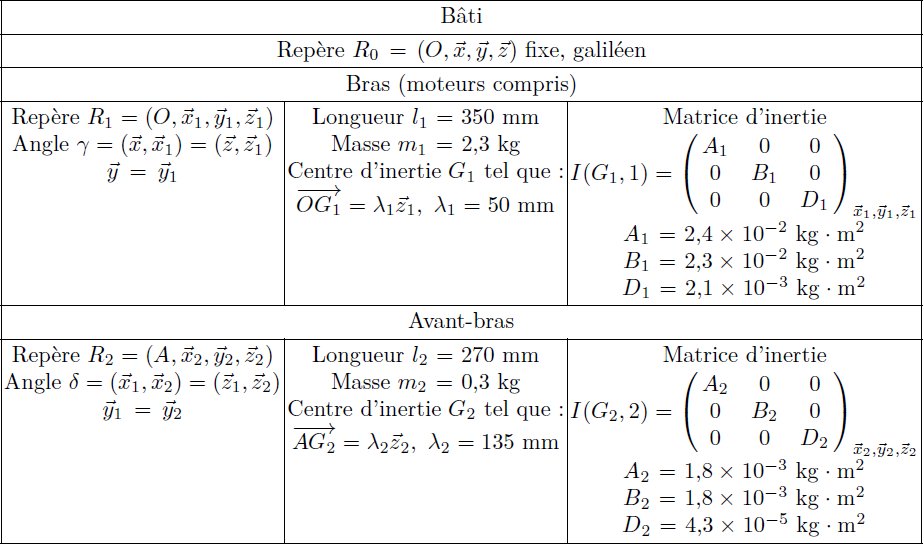
\includegraphics[width=1.0\linewidth]{fig_06}
\end{center}


\subparagraph{}\textit{Montrer que les deux équations précédentes peuvent s'écrire sous la forme matricielle suivante : 
$\begin{pmatrix}
C_1 \\ C_2
\end{pmatrix}
=
A
\begin{pmatrix}
\ddot{\gamma} \\ \ddot{\delta}
\end{pmatrix}
+
B
\begin{pmatrix}
\dot{\gamma} \\ \dot{\delta}
\end{pmatrix}
+
C
+
Q
\begin{pmatrix}
X_F \\ Z_F
\end{pmatrix}$ où $C$ est un vecteur et $A$, $B$ et $Q$ sont des matrices $2\times 2$ que l'on précisera en fonction des paramètres du mouvement $\left(\gamma,\delta\right)$ et de leurs dérivées premières $\left(\dot{\gamma},\dot{\delta}\right)$.
}

\ifprof
\begin{corrige}
\end{corrige}
\else
\fi


\question{Calculer les couples $(C_1,C_2)$ exercés par les actionneurs sur les axes des articulations dans le cas où
l’on n’exerce pas de force à l’extrémité du solide \{Avant-bras\} ($X_F = 0$, $Z_F = 0$) et dans une position statique. Discuter de la configuration angulaire la plus défavorable vis-à-vis du cahier des charges.}
\ifprof
\begin{corrige}
\end{corrige}
\else
\fi


\question{Compte-tenu du cahier des charges, quelle charge statique maximale peut-on exercer sur l’extrémité du solide \{Avant-bras\} ?}
\ifprof
\begin{corrige}
\end{corrige}
\else
\fi



\subsection*{Synthèse d’une loi de commande « deux axes »}

\begin{obj}
L’objectif de cette partie est de déterminer une loi de commande afin que la relation entre les variations
des positions $ ^t\left(\gamma,\delta\right)$ du bras et de l’avant-bras, et la variation de la force $Z_F$ exercée par le patient soit celle d’une raideur en torsion de valeurs $(K_1;K_2)$ données dans le cahier des charges. La raideur comparativement à la force $X_F$ ne sera pas à vérifier dans ce cas d’étude.
\end{obj}


L’équation dynamique décrivant le comportement de l’exosquelette est de la forme 
$A(q, \dot{q})\ddot{q}+ B(q, \dot{q})\dot{q} + C(q, \dot{q}) + Q(q, \dot{q}) F = C_a$ 
où $C_a = ^t(C_1\quad C_2)$, $q = ^t(\gamma \quad \delta)$ et $F = ^t(X_F \quad Z_F )$. On note sous forme vectorielle $q_{\text{ref}} = ^t(\gamma_{\text{ref}} \quad \delta_{\text{ref}})$ les consignes
de positions angulaires. La loi de commande adoptée est organisée selon deux boucles :
\begin{itemize}
\item une boucle externe linéaire ;
\item une boucle interne non linéaire qui détermine le couple $C_a$ par la relation
$C_a = B(q, \dot{q})\dot{q} + C(q, \dot{q}) + A(q, \dot{q}) U$.
\end{itemize}
où $U = ^t(U_1 \quad U_2)$ sont les deux nouvelles commandes issues du correcteur linéaire de la boucle externe.

Le principe de cette loi de commande est donné par la structure représentée par le schéma suivant.

\begin{center}
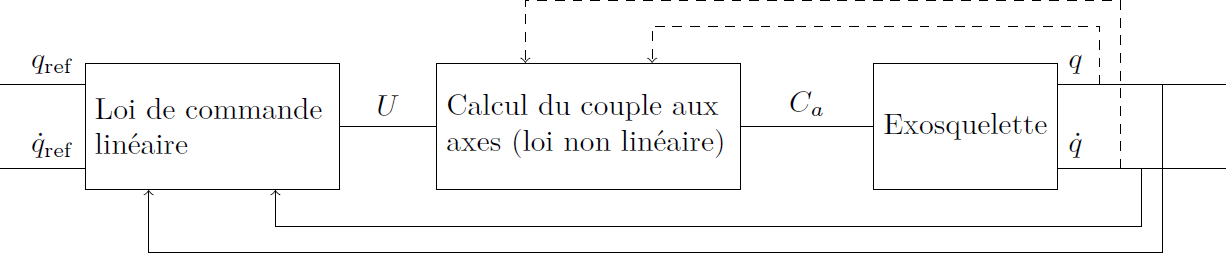
\includegraphics[width=1.0\linewidth]{fig_07}
\end{center}

\question{Donner au moins un argument, en particulier vis-à-vis du cahier des charges souhaité, de l’intérêt de la
boucle interne correspondant à la loi non linéaire donnée précédemment.}

Pour la synthèse de la loi de commande, il est nécessaire de linéariser le modèle dynamique autour d’un point
de fonctionnement défini par les positions articulaires $ ^t(\gamma_0 \quad \delta_0)$ et les forces $ ^t\left(X_{F0}\quad Z_{F0}\right)$. On note autour de ce point de fonctionnement :
\begin{itemize}
\item $ u = ^t\left(u_1\quad u_2\right)$ les variations des grandeurs de commande autour de $ U_0 = ^t\left(U_{10}\quad U_{20}\right)$;
\item $q_1 = ^t\left(\gamma_1 \quad \delta_1\right)$ les variations des positions angulaires des deux articulations autour de $q_0 = ^t\left(\gamma_0 \quad \delta_0\right)$;
\item $ f = ^t\left(x_F \quad z_F \right)$ les variations des efforts exercés par le patient autour de $F_0 =  ^t\left(X_{F0} \quad Z_{F0} \right)$.
\end{itemize}
En utilisant la loi correspondant à la boucle interne, le modèle dynamique peut-être réécrit selon la forme
$\ddot{q}= U + N\left(q, \dot{q}, F\right)$, où $N\left(q, \dot{q}, F\right) = M\left(q, \dot{q}\right) F$.



\question{Préciser l’expression de la matrice $M$ en fonction de $A$ et de $Q$.}
\ifprof
\begin{corrige}
\end{corrige}
\else
\fi



\question{Donner, par exemple sous forme algorithmique, une démarche permettant de linéariser le modèle dynamique selon la forme $\ddot{q}_1 = \tilde{A}q_1+\tilde{B}\dot{q}_1+\tilde{G}u+\tilde{H}f$ où $\tilde{A}$, $\tilde{B}$, $\tilde{G}$ et $\tilde{H}$ sont des matrices constantes, éventuellement
dépendantes du point de fonctionnement.}
\ifprof
\begin{corrige}
\end{corrige}
\else
\fi


Indication : la démarche de linéarisation fait intervenir $\dfrac{\partial N}{\partial q}$, $\dfrac{\partial N}{\partial \dot{q}}$ et $\dfrac{\partial N}{\partial F}$; l’expression explicite du modèle linéarisé
en fonction de $M$ n’est pas demandée.


On admet pour la suite que le modèle linéarisé, décrivant les variations des positions $ ^t\left(\gamma_1 \quad \delta_1 \right)$ du bras, autour du point de fonctionnement $q_0 = ^t\left(0,6 0,7\right)$ rad et $F_0 = ^t\left(0 \quad -5\right)$ N, est représenté par le système d’équations différentielles suivantes :


$$
\begin{pmatrix}
\ddot{\gamma_1} \\
\ddot{\delta_1}
\end{pmatrix}
=
\begin{pmatrix}
-18,4 & -33 \\
4 & -56,5
\ddot{\delta_1}
\end{pmatrix}
\begin{pmatrix}
{\gamma_1} \\
{\delta_1}
\end{pmatrix}
+
\begin{pmatrix}
\ddot{u_1} \\
\ddot{u_2}
\end{pmatrix}
+
\begin{pmatrix}
-3,9 \\
-45,4
\end{pmatrix}
z_F.
$$

On note $q_{1\text{ref}} = ^t\left(\gamma_{\text{ref}}, \delta_{\text{ref}} \right)$ les variations de consignes de position. L’objectif des questions suivantes est la
synthèse d’une loi de commande linéaire en vue d’assurer la raideur souhaitée entre les variations des positions  $ ^t\left(\gamma_{1}, \delta_{1} \right)$ des deux articulations et la variation de l’effort $z_F$ exercé par le patient. L’adaptation de la loi de
commande au point de fonctionnement ne fait pas partie du cadre de cette étude.




\question{En justifiant la réponse, étudier la stabilité du modèle donné ci-dessus.}
\ifprof
\begin{corrige}
\end{corrige}
\else
\fi


\question{En utilisant un raisonnement qualitatif (sans calcul), et en supposant que le système bouclé est stable, justifier qu’une régulation de type proportionnelle-intégrale (sur chaque composante des positions du bras) :
$\dfrac{U_1(p)}{\varepsilon_1(p)}=K_1\left(1+\dfrac{1}{T_1 p}\right)$
et
$\dfrac{U_2(p)}{\varepsilon_2(p)}=K_2\left(1+\dfrac{1}{T_2 p}\right)$
où $\varepsilon_1(p)=\gamma_{1\text{ref}}-\gamma_1$
et $\varepsilon_2(p)=\delta_{1\text{ref}}-\delta_1$ sont les écarts sur chaque axe d’articulation étudié, ne permet pas
d’assurer l’objectif escompté, c’est-à-dire un comportement de type raideur entre les variations des positions 
$\gamma_1$ et $\delta_1$, du bras et de l’avant-bras, et la variation de la force $z_F$ exercée par le patient.
}
\ifprof
\begin{corrige}
\end{corrige}
\else
\fi

Pour la suite, on adopte la loi de commande $u(t)=K_p \left(q_{1\text{ref}}-q_1\right)+K_v \left(\dot{q}_{1\text{ref}}-\dot{q}_1\right)$ avec :

$$
K_p = \begin{pmatrix} 
k_{p11} & k_{p12} \\
k_{p21} & k_{p22}
\end{pmatrix}
\quad
\text{et}
\quad 
K_v = \begin{pmatrix} 
k_{v11} & k_{v12} \\
k_{v21} & k_{v22}
\end{pmatrix}.
$$

Par souci de simplicité, on pourra utiliser $q_{1\text{ref}}=0$ et $\dot{q}_{1\text{ref}}=0$.



\question{Déterminer les coefficients des matrices $K_p$ et $K_v$ afin que le comportement entrée-sortie entre les positions du bras et de l’avant bras, et les forces exercées par le patient, soit celui de fonctions du deuxième ordre :
$\dfrac{\gamma_1(p)}{Z_F(p)}=\dfrac{K_1}{1+\dfrac{2\xi}{\omega_1}p+\dfrac{p^2}{\omega_1^2}}$ 
et 
$\dfrac{\delta_1(p)}{Z_F(p)}=\dfrac{K_2}{1+\dfrac{2\xi}{\omega_2}p+\dfrac{p^2}{\omega_2^2}}$
permettant d’obtenir les valeurs des raideurs souhaitées et caractérisées par un coefficient d’amortissement
$\xi = 0,7$. Justifier alors que la bande passante ne peut pas être choisie d’une manière arbitraire.
}
\ifprof
\begin{corrige}
\end{corrige}
\else
\fi


Les figures suivantes montrent un ensemble de résultats correspondant à deux types d’essais :
\begin{itemize}
\item pour le réglage de la loi de commande correspondant à celui de la question précédente, la première figure suivante montre les évolutions des positions angulaires du bras et de l’avant-bras (à partir du point de fonctionnement $ ^t(0,6 \quad 0,7)$ rad)
et des couples sur les axes des articulations, en réponse à une variation intervenant à $t_0 = \SI{1}{s}$ de la force $z_F = \Delta Z_F = -\SI{1}{N}$;
\item la seconde figure montre le ralliement à une position de référence avec des efforts constants, $X_F = \SI{50}{N}$ et $Z_F = -\SI{50}{N}$ en partant de conditions initiales nulles.
\end{itemize}
\question{Commenter ces courbes et conclure sur l’adéquation de la loi de commande proposée comparativement au cahier
des charges.}
\ifprof
\begin{corrige}
\end{corrige}
\else
\fi



\end{multicols}

\begin{center}
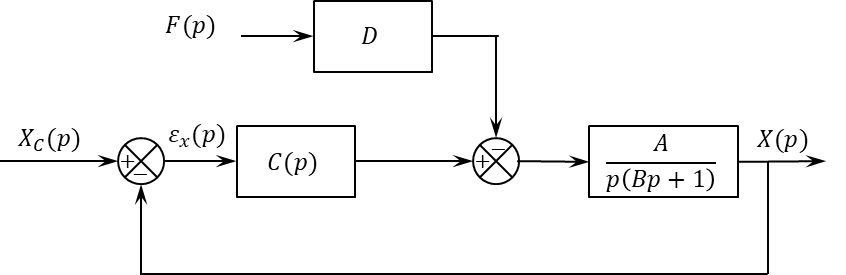
\includegraphics[width=1.0\linewidth]{fig_08}
\end{center}
